\newpage
\subsection{Lineare elektrische Netzwerke}
\begin{minipage}{0.35\textwidth}
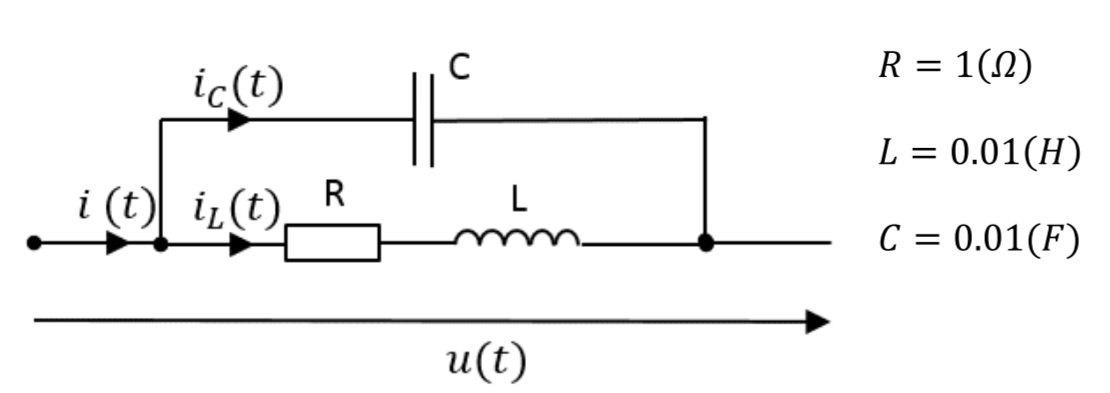
\includegraphics[width=0.9\textwidth]{bilder/a31.png}
\end{minipage}
\begin{minipage}{0.64\textwidth}
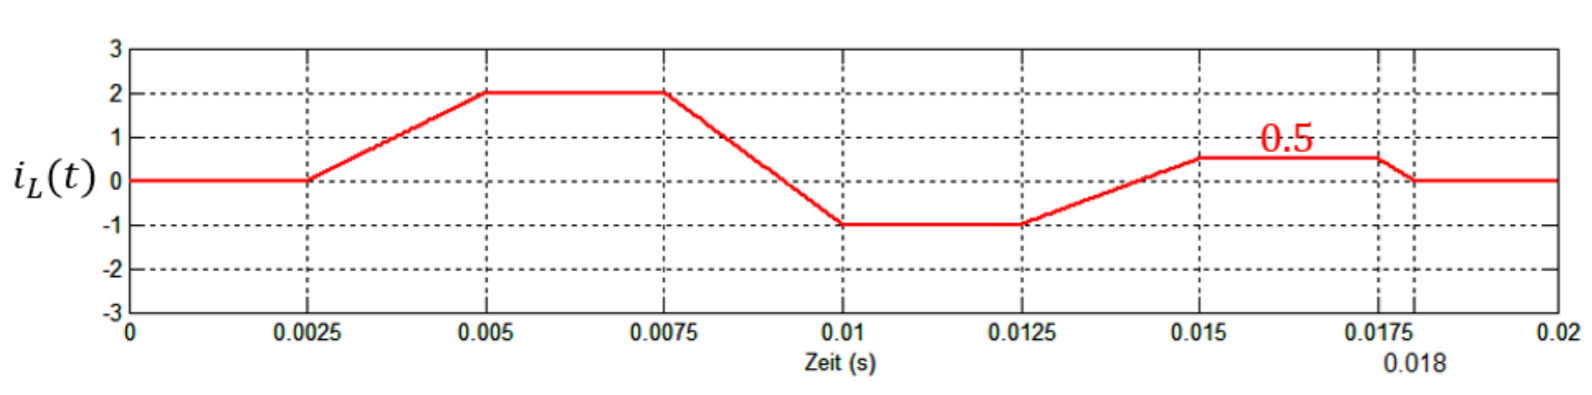
\includegraphics[width=0.9\textwidth]{bilder/a32.png}
\end{minipage}

Die gegebenen Ströme sind die Ströme über dem Spulenpfad. Die Funktionen sind gemäss Aufgaben 1 auf Seite \pageref{ueb1}

Gesucht sind \begin{itemize}
\itemsep0em
\item $u(t)$
\item $i_c(t)$
\item $i(t)$
\item Eintrag ins Diagramm
\end{itemize}

\begin{minipage}{0.49\textwidth}
\begin{align*}
u(t)&=R\cdot i(t)+L\cdot \frac{di}{dt}\\
u_1(t)&=0&&=0\\
u_2(t)&=800\cdot t -2+0.01\cdot 800&&=800\cdot t+6\\
u_3(t)&=2&&=2\\
u_4(t)&=-1200\cdot t+11 +0.01\cdot (-1200)&&=-1200\cdot t -1\\
\vdots&=\vdots
\end{align*}
\end{minipage}
\begin{minipage}{0.49\textwidth}
\begin{align*}
i_c&= C\cdot \frac{du}{dt}\\
i_1(t)&=0&&=0\\
i_2(t)&=0.01\cdot 800&&=8\\
i_3(t)&=0&&=0\\
i_4(t)&=0.01\cdot (-1200)&&=-12\\
\vdots&=\vdots
\end{align*}
\end{minipage}
\vspace{5mm}
$i(t)$ ist nun nur die Summe der Serieschaltung und des Kondensators: $i(t) = i_c(t) + i_L(t)$

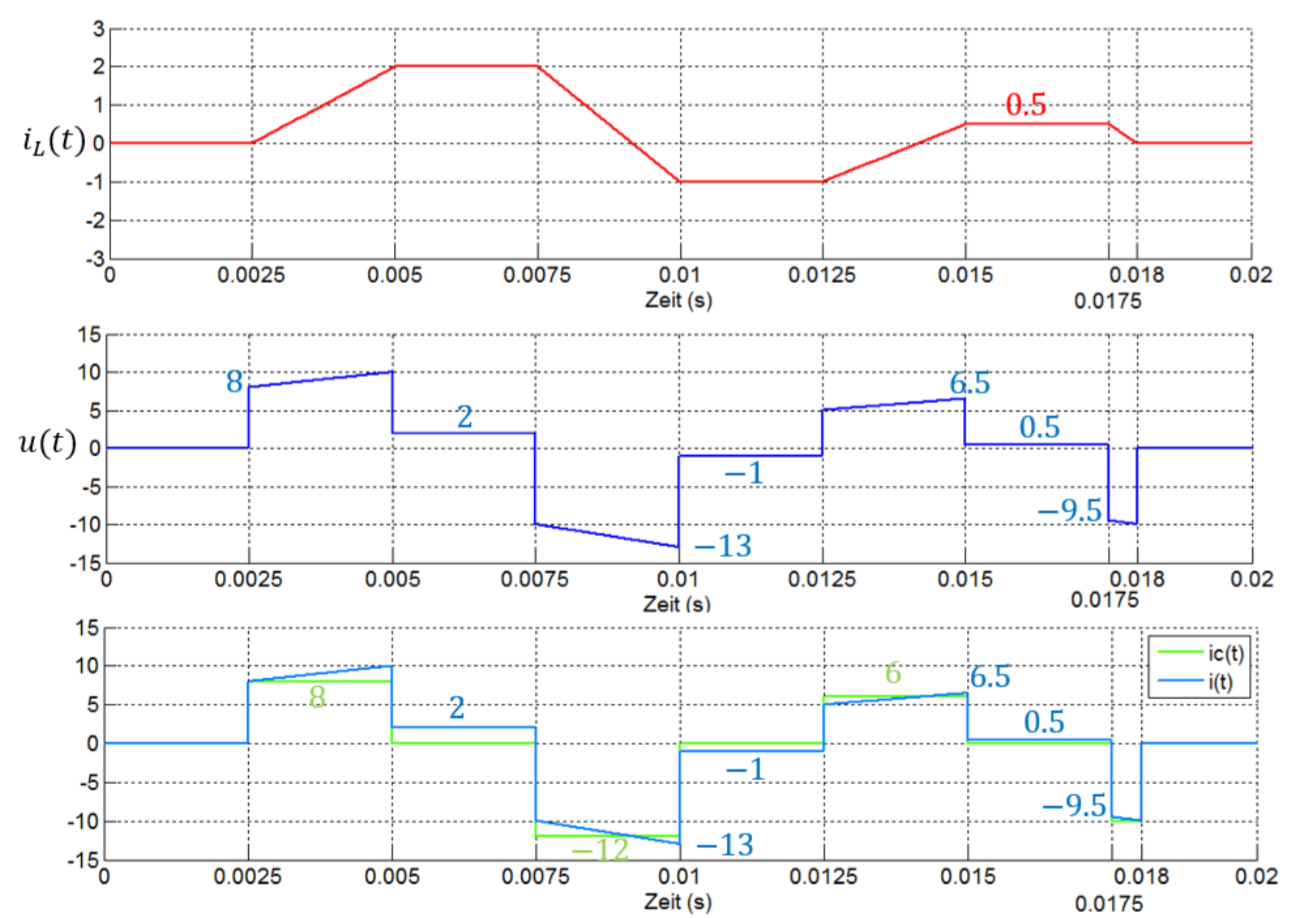
\includegraphics[width=0.95\textwidth]{bilder/a33.png}
